%%%%%%%%%%%%%%%%%%%%%%%%%%%%%%%%%%%%%%%%%%%%%%%%%%%%%%%%%%%%%%%%%%%%%%
%% On jet mass corrections and transversity
%% May 10, 2013
%%%%%%%%%%%%%%%%%%%%%%%%%%%%%%%%%%%%%%%%%%%%%%%%%%%%%%%%%%%%%%%%%%%%%%
\documentclass[preprintnumbers,floatfix,nofootinbib]{revtex4}

\usepackage[tbtags]{amsmath}  % AMS math 
\usepackage{amssymb}          % AMS symbols
\usepackage{bm}               % bold math
\usepackage{graphicx}         % PostScript figures
\usepackage[export]{adjustbox}% to align images
\usepackage{hhline,multirow}  % for nicer tables
\usepackage{dcolumn}          % Align table columns on decimal point
\usepackage{slashed}
\usepackage{datetime}
\usepackage{color}
\usepackage[dvipsnames]{xcolor}

%%%%%% for draft
\newcommand{\todo}[1]{\marginpar{$\bullet$}\textbf{#1}}
\def\AAcom#1{{\bf  \textcolor{Red}{[AA: {#1}]}}}
\def\AAmod#1{{\textcolor{Green}{#1}}}

%%%%%%  Definitions   %%%%%%%%%%%
  
\newcommand{\Pslash}{P \hspace{-0.24cm} / \,}
\newcommand{\kslash}{k \hspace{-0.21cm} / \,}
\newcommand{\lslash}{l \hspace{-0.19cm} / \,}
\newcommand{\nslash}{n \hspace{-0.24cm} / \,}
\newcommand{\vslash}{v \hspace{-0.21cm} / \,}
\newcommand{\Sslash}{S \hspace{-0.22cm} / \,}
\newcommand{\Dslash}{D \hspace{-0.22cm} / \,}
\newcommand{\epsslash}{\varepsilon \hspace{-0.18cm} / \,}
\newcommand{\Tr}{\operatorname*{Tr}\nolimits} % Trace operator
\newcommand{\xbj}{x}                   % Bjorken variable
\newcommand{\de}{d}                    % differential
\newcommand{\ii}{i}                    % imaginary unit

%\newcommand{\mj}{\langle m_j \rangle}
%\newcommand{\mj}{M_q^\text{jet}}
\newcommand{\mj}{M_q}
\newcommand{\mjs}{\langle m_j^2 \rangle>}

\allowdisplaybreaks[2]

\begin{document}

%%%%%%%%%%%%%%%%%%%%%%%%%%%%%%%%%%%%%%%%%%%%%%%%%%%%%%%%%%%%%%%%%%%%%%
%%%%%%%%%%%%%%%%%%%%%%%   TITLE    %%%%%%%%%%%%%%%%%%%%%%%%%%%%%%%%%%%
%%%%%%%%%%%%%%%%%%%%%%%%%%%%%%%%%%%%%%%%%%%%%%%%%%%%%%%%%%%%%%%%%%%%%%

\preprint{JLAB-THY-13-????}

\title{Accessing the nucleon tensor structure in inclusive deep inelastic scattering} 

\author{Alberto~Accardi$^{a}$, Alessandro~Bacchetta$^{b}$} 
\affiliation{
$^a$Jefferson Lab, Newport News, VA 23606, USA, and
Hampton University, Hampton, VA 23668, USA \\
$^b$Dipartimento di Fisica, Universit\`a degli Studi di Pavia, and INFN,
Sez. di Pavia, 27100 Pavia, Italy
}

\date{\today, \currenttime}

\begin{abstract}

\end{abstract}

%\pacs{ }

%\keywords{ }

\maketitle


%%%%%%%%%%%%%%%%%%%%%%%%%%%%%%%%%%%%%%%%%%%%%%%%%%%%%%%%%%%%%%%%%%%%%%%%%
\section{Introduction}

%%%%%%%%%%%%%%%%%%%%%%%%%%%%%%%%%%%%%%%%%%%%%%%%%%%%%%%%%%%%%%%%%%%%%%%%%
\section{Jet correlator and twist-2 structure functions}

Motivated by large-$x$ mass corrections to inclusive DIS structure functions, Accardi and Qiu have introduced in the LO handbag diagram a ``jet correlator'' that accounts for invariant mass production in the current jet, and ensures that leading twist calculations in collinear factorization are consistent with the requirement imposed by baryon number conservation that $x_B<1$ \cite{Accardi-Qiu}. The jet correlator is depicted in Figure~\ref{fig:handbags}(a) and is defined as
\begin{align} 
\Xi_{ij}(l,n_+) =\int
  \frac{\de^4\eta}{(2\pi)^4}\; e^{i l \cdot \eta}\,
    \langle 0|\, {\cal U}^{n_+}_{(+\infty,\eta)}
\,\psi_i(\eta)
             \bar{\psi}_j(0)\,
{\cal U}^{n_+}_{(0,+\infty)}\,   |0 \rangle \ ,
\label{e:xifull}
\end{align} 
In this definition, $l$ is the quark four-momentum, $\Psi$ the quark field operator, and $\|0\rangle$ is the nonperturbative vacuum. Furthermore, we explicitly guarantee the correlator's gauge invariance by introducing two Wilson line operators ${\cal U}^{n_+}$ along a light-cone plus direction determined by the vector $n_+$. This path choice for the Wilson line is required by QCD factorization theorems, and the vector will be determined by the particular hard process to which the jet correlator contributes. For example, in the case of inclusive DIS discussed in this paper, this is determined by the four momentum transfer $q$ and the proton's momentum $p$.

\begin{figure*}
  \centering
  (a)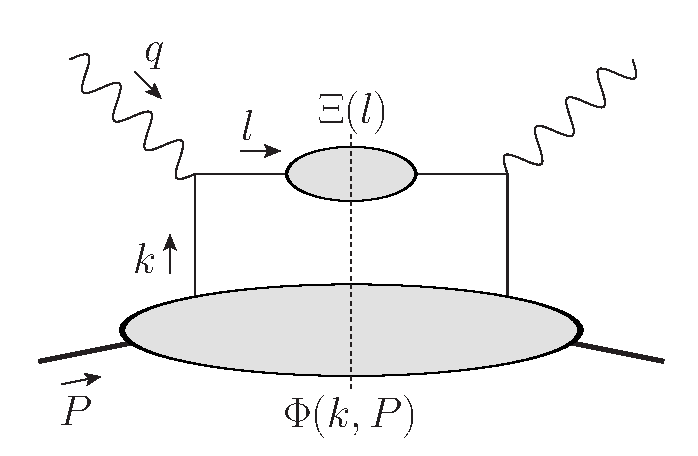
\includegraphics[width=0.3\linewidth,valign=t]{jetdiagram0}
  \hfill
  (b)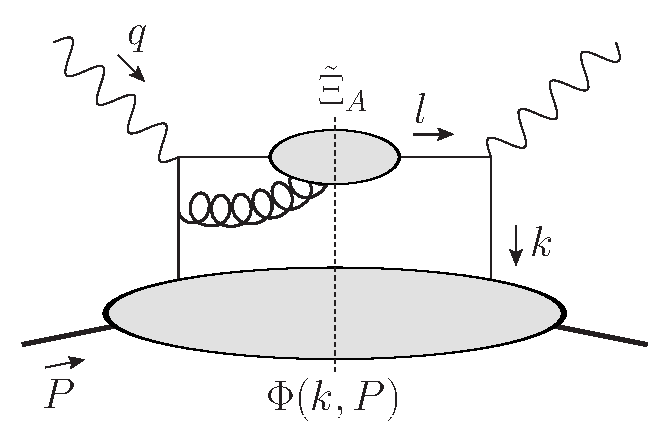
\includegraphics[width=0.3\linewidth,valign=t]{jetdiagram1}
  \hfill
  (c)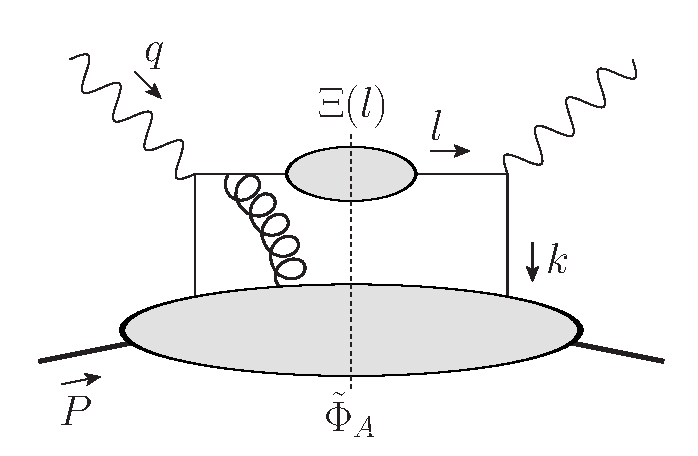
\includegraphics[width=0.3\linewidth,valign=t]{jetdiagram2}
  \caption{Diagrams contributing to DIS scattering up to twist-3 expansion, including a jet correlator in the top part. Note the gluon attaches to both the nucleon and jet correlators. The Hermitian conjugates of diagrams (b) and (c), i.e., with gluons attaching to the right of the cut, are not shown.
  }
  \label{fig:handbags}
\end{figure*}

The correlator $\Xi$ can be parametrized in terms of scalar functions, using the vectors $l$ and $n_+$ 
\begin{equation}
\Xi(l,n_+) = \Lambda A_1(l^2)\,{\bm 1} + A_2(l^2)\,\lslash 
+ \frac{\Lambda^2}{l \cdot n_{+}} \nslash_+ \, B_{1}(l^2)
+ \frac{i \Lambda}{2 P \cdot n_{+}} [\,\lslash,\nslash_+ ] \, B_{2}(l^2) \ .
\label{e:jetexpansion}
\end{equation} 
Time reversal invariance in QCD requires $B_{2}=0$, while $B_{1}$ contributes
only at twist-4 order, and will not be considered further in this paper. We
focus on the role of chiral odd terms in the $g_2$ structure function up to
twist 3.  At this order, 
\begin{equation}
  \Xi(l,n_+) = \Lambda A_1(l^2)\,{\bm 1} + A_2(l^2)\,\lslash 
    + O(\Lambda^2/Q^2)
\label{e:jetexpansion-tw3}
\end{equation} 
is nothing else than the full quark propagator; note however, that we consider
here the full QCD vacuum rather than the perturbative one.  

The $A_1$ and $A_2$ terms can be nicely interpreted in terms of the spectral representation of the cut quark propagator,
\begin{align} 
  \Xi(l) =  
  \int d \mu^2 \big[ J_1 (\mu^2)\,\mu + J_2 (\mu^2)\,\lslash \big] \,
  \delta(l^2 -\mu_j^2) \ ,
\label{e:jetspectral}
\end{align}
where $\mu^2$ is interpreted as the invariant mass of the current jet, {\it i.e.}, of the particles going through the cut in the top blob of Fig.\ref{fig:handabgs}(a), and the $J_i$ are the spectral functions of the quark propagator, that have been also called ``jet functions'' in \cite{Accardi-Qiu}. These satisfy \cite{D'Hoker-lecture-notes,Romao-lecture-notes}
\begin{align}
  J_2(\mu^2) \geq J_1(\mu^2) \geq 0
  \hspace*{0.5cm} \text{and} \hspace*{0.5cm}
  \int d\mu^2 J_2(\mu^2) = 1 \ .
\label{eq:jetfnsprops}
\end{align}
From a comparison of Eqns.\eqref{e:jetexpansion} and \eqref{e:jetspectral}, one can see that 
\begin{align}
  A_1(l^2)&=\frac{\sqrt{l^2}}{\Lambda}J_1(l^2) & A_2(l^2)&=J_2(l^2) \ .
  \label{eq:jet_vs_spectral}
\end{align}

When inserting the jet correlator in the handbag diagram for inclusive DIS, the invariant jet mass $\mu^2$ is integrated from 0 to $Q^2(1/x_B-1)$. This induces (kinematical) corrections of order $O(1/Q^2)$, whose effect on the $F_2$ structure function has been studied in Ref.~\cite{Accardi-Qiu}; for example, 
teh structure function $F_2$ reads
\begin{align}
  F_2(x_B) & = \int_0^{Q^2(1/x_B-1)}d\mu^2\, J_2(\mu^2) F_2^{(0)}(x_B(1+\mu^2/Q^2),Q^2) \ ,
\label{eq:F2}
\end{align}
where $F_2^{(0)}$ is the structure function calculated with the handbag diagram sporting a bare quark propagator instead of the jet correlator, and $\xi=2x_B/(1+\sqrt{1+4x_B^2M^2/Q^2})$ with $M$ the nucleon's mass is the Nachtmann scaling variable.  In this paper we limit our attention to effects of order $O(1/Q)$ and therefore can extend the integration to $\mu^2=\infty$. Therefore jet function $J_2$ decouples, and thanks to the sum rule \eqref{eq:jetfnsprops} integrates to 1. One then recovers the conventional result.
\begin{align}
  F_2(x_B) = \Big[ \int_0^\infty d\mu^2\, J_2(\mu^2) \Big] F_2^{(0)}(x_B,Q^2) 
     + O(\Lambda^2/Q^2) = F_2^{(0)}(x_B,Q^2)  + O(\Lambda^2/Q^2) \ .
\end{align}
The same holds true also for the helicity structure function $g_1$.
%
More in general, the jet correlator decouples from the parton correlator $\Phi$ in any inclusive cross section calculation up to $O(1/Q)$, and the inclusive structure functions only depend on the integrated jet correlator
\begin{equation} 
  \Xi(l^-) \equiv \int \frac{dl^2}{2l^-} d^2 l_T \, \Xi(l) 
    =  \frac{\Lambda}{2 l^-}\,\xi_1 {\bm 1}
    +  \xi_2 \frac{\nslash_-}{2} 
    + \text{higher\ twists}
    % +\frac{\Lambda^2}{4 (l^-)^2}\,\xi_3 \nslash_+
    % + i \frac{\Lambda}{2 l^-} \xi_4 
    % \frac{ \bigl[\nslash_-, \nslash_+ \bigr]}{2}.
\end{equation} 
\AAcom{We need to discuss what happens to the B functions!! See e-mail from Jul 7th, 2015, for ideas.}
where 
\begin{align}
\xi_1 &= \int d\mu^2 \frac{\mu}{\Lambda} J_1(\mu^2) 
       \equiv \frac{\mj}{\Lambda},
&
\xi_2 &= \int d\mu^2 J_2(\mu^2) = 1 \ .
% \\
% \xi_3 &= 0,
% &
% \xi_4 &= \int d\mu^2 \frac{\mu^2}{\Lambda^2} J_1(\mu^2) = \frac{\mjs}{\Lambda^2}.
\end{align} 
% The $\xi_1$ and $\xi_4$ have an interpretation as average invariant mass (and mass squared) of the current jet, and $l^-=q^- + O(1/Q)$ is imposed by 4-momentum conservation at the hard scattering vertex. The $\xi^4$ term contributes at order $O(1/Q^2)$ and is no further considered in this paper. 
It is important to notice that $\xi_2=1$ exactly due to CPT invariance \cite{Weinberg-book}, while $0 < M_q < \int d\mu^2 \mu J_2(\mu^2)$ is dynamically determined. From the analytic properties of spectral functions we may expect \cite{Accardi-Qiu)} $J_2(\mu^2) = Z \delta(\mu^2-m_q) + \bar J_2 (\mu^2) \theta (\mu^2-m_\pi)$ with the continuum starting at $m_\pi$, the mass of the pion, due to color confinement effects. Taking into account that $J_1 < J_2$, we may therefore expect 
\begin{align}
  \label{eq:mjet}
  \mj = O(10-100 \text{ MeV}) \ .
\end{align}
Although $\mj$ is in general a nonperturbative quantity, it is interesting to
notice that  
\begin{align}
  \label{eq:xi2_chiral_cond}
  \mj = \frac{\Lambda}{4} \int \Tr \big[ \Xi(l) \bm 1] 
   = \langle 0 | \bar \psi_i(0) \psi_i(0) | 0 \rangle
\end{align}
% \todo{[AA] 2 issues here: (1) possible factors of 4. 
% (2) I am neglecting the sum over quarks; we have to fix that somehow but there is a little tension between the quark level $\xi^a$ and the contribution to structure function which is summed and weighted by the electron charge.} 
Calculating this on the perturbative vacuum and limiting oneself to LO
corresponds to taking the trace of the cut bare-quark propagator to obtain 
$\mj = \,_{\text{pert}} \langle 0
|  \bar \psi_i(0) \psi_i(0) | 0 \rangle_{\text{pert}}  = m_q$, recovering the
conventional result. However, we are here considering non perturbative effects
on the quark fragmentation and $\mj \gtrsim m_q$. 
%very importantly, this
%quantity can be computed in lattice QCD. 
%\todo{[AA] Are qe sure that $\mj > m_q$??}
%\todo{[AA] Need to discuss connection to quark condensate and tensor charge.}

\section{Twist-3 analysis}

Extending the analysis of \cite{Accardi-Qiu} to the calculation of twist-3
structure functions requires not only to consider the $\xi_1$ term in the jet
correlator, but also quark-gluon-quark correlators in both the proton and the
vacuum as depicted in Figs.\ref{fig:handbags}(b) and (c), respectively. 
In the former the $\xi_1$ terms contribute to $O(1/Q^2)$, so that up $O(1/Q)$
these give the same contribution as in the conventional handbag calculation.  

The novel element in our analysis is the jet quark-gluon quark correlators
$\Xi_A^{\mu}(l,k)$ in diagrams \ref{fig:handbags}(c), 
\begin{equation} 
\begin{split} 
  \left(\Xi_A^{\mu} \right)_{ij} &=
   \frac{1}{2}\, \sum_X \int \frac{\de \eta^+\, \de^2 \bm{\eta}_T}{(2\pi)^{3}}\;
   e^{\ii k \cdot \eta}\,
   \langle 0|\,
   {\cal U}^{n_+}_{(+\infty,\eta)}\,
   g A^{\mu}(\eta)\,
   \,\psi_i(\eta)|X\rangle
   \langle X|
             \bar{\psi}_j(0)\,
   {\cal U}^{n_+}_{(0,+\infty)}
   |0\rangle \bigg|_{\eta^-=0} .
\label{e:xi_A}
\end{split} 
\end{equation}  
These diagrams are not only important to account for all contribution of order $O(1/Q)$, but also in restoring up to twist-3 the gauge invariance broken in diagram \ref{fig:handbags}(a) by the different mass of the incoming and outgoing quark lines, namely, $m_q \neq \mj$.

Rather than directly using the definition \eqref{e:xi_A}, it is convenient to calculate the inclusive cross section as an integral of the semi-inclusive one, utilize the QCD equation of motions and furthermore summed over all hadron flavors, and take advantage of 
\begin{align}
  \label{eq:SIDIS_to_DIS}
  \sum_h \int \frac{d^3p_h}{(2\pi)2E_h} \Delta^h(l,p_h) = \Xi(l) \ , 
\end{align}
where $\Delta^h$ is the quark fragmentation correlator for production of a hadron of flavor $h$ and momentum $p_h$ \cite{New_testament}. 
% As we shall see, an analogous formula for quark-gluon-quark correlators is not needed.
The $\xi_1$ term is chiral-odd and therefore can appear in the inclusive cross section only coupled to the transversity function $h_1$. Therefore, for our analysis the relevant part of the semi-inclusive hadronic tensor is 
\todo{[AA] I am using the notation in Piet Mulder's lecture notes - this will need to be checked. Decide also if we want this at parton or charge-weighted level.}
\begin{align}
  \label{eq:Wsidis_ini}
  2 \Lambda \sum_h \int dz d^2p_{hT} = i \frac{2\Lambda}{Q} 
    \hat t^{[\mu} \epsilon_\perp^{\nu]\rho}S_{\perp\rho} 
    \Big[ 2 x_b g_T(x_B) \sum_h \int dz d^2p_{hT} D_1^h(z)
    + 2 h_1(x_B) \sum_h \int dz d^2p_{hT} \tilde E^h(z) \Big] + \ldots
\end{align}
where $D_1^h$ is the twist-2 quark fragmentation function as a function of the hadron's collinear momentum fraction $z$, and $\tilde E^h$ is a twist-3 function defined in \cite{New-testament}. The former can be easily integrated with the help of the sum rule \eqref{eq:SIDIS_to_DIS}:
\begin{align}
  \sum_h \int dz d^2p_{hT} z D_1^h(z) = \xi_2 = 1 \ .
\end{align}
To integrate the latter, we first make use of the relation \cite{New-testament}
$\tilde E(z) = E(z) - m_q z D_1(z)$, which is a consequence of the QCD equations of motion, so that 
\begin{align}
  \sum_h \int dz d^2p_{hT} \tilde E(z) 
    = \sum_h \int dz d^2p_{hT} \Big[ E(z) - \frac{m_q}{\Lambda} z D_1z \Big]
    = \xi_1 - \frac{m_q}{\Lambda} \xi_2 = \frac{\mj - m_q}{\Lambda} \ .
\end{align}
This formula is the single most important result of this paper.

Finally, with suitable projections of the hadronic tensor, the inclusive cross section up to order $M/Q$ turns out to be
\begin{align}
\frac{d\sigma}{d\xbj \, dy\, d\psi}
%&
=
\frac{2 \alpha^2}{\xbj y Q^2}\,
\frac{y^2}{2\,(1-\varepsilon)}\, 
\biggl\{
&F_{UU ,T} + \varepsilon F_{UU ,L}
+ S_\parallel \lambda_e\,
  \sqrt{1-\varepsilon^2}\; 
F_{LL}
%\nonumber 
\\  
&
+ |\bm{S}_\perp| \lambda_e\, \sqrt{2\,\varepsilon (1-\varepsilon)}\, 
  \cos\phi_S\, 
F_{LT}^{\cos \phi_S}
 \biggr\},
\label{e:crossdis}
\end{align}
where the structure functions on the right hand side are defined as
\begin{align}
F_{UU ,T} &= \xbj\,\sum_a e_a^2\,f_1^a(\xbj),
\\
F_{UU ,L} &= 0,
\\
F_{LL} &=\xbj\,\sum_a e_a^2\,g_1^a(\xbj),
\\
F_{UT}^{\sin \phi_S}&=0,
\label{e:FUTint}
\\
F_{LT}^{\cos \phi_S}&=-\xbj\,\sum_a e_a^2\, \frac{2\Lambda}{Q}\,
\biggl(\xbj  g_T^a(\xbj)
   + \frac{\mj -m_q}{\Lambda} \, h_{1}^a(\xbj) \biggr).
\label{e:FLTint}
\end{align}
The second term in the last struture function is a new result from our
analysis; it is not suppressed as an inverse power of $Q$, and therefore
survives even in the Bjorken limit. Note that calculating the jet correlator
on the perturbative vacuum one would obtain, as already discussed, $\mj=m_q$
and the new term vanishes as it should. However, on the non-perturbative
vacuum the jet mass is larger than the quark's, and this contributes a
non-negligible term to the twist-3 part of the $g_2$ function, as we shall
discuss in the next section.  

 

\section{The $g_2$ structure function}

The new term in Eq.{e:FLTint} only appeears in the $g_2$ structure function. Following the derivation in Ref.~\cite{ABMS}, one finds
\begin{align}
\label{e:g2}
  g_2(x_B) = g_2^{WW} + \frac{1}{2}\,\sum_a e_a^2
\biggl(
    \widetilde g_T^{a \star}(x) 
    + \int_x^1\frac{dy}{y} \widehat{g}_T^a(y) 
    + \frac{m_q}{M} (h_1^a/x)^\star(x) 
    + \frac{\mj-m_q}{M} h_1^a(x) 
\Biggr) \ ,
\end{align}
where we defined $f^*(x) = -f(x) + \int_x^1\frac{dy}{y} f(y)$. The first 4
terms coincide with the result obtained in the conventional handbag
approximation \cite{ABMS}, while the fifth is new. 

The first term is also known as the Wandzura-Wilczeck function $g_2^{WW} =
g_1^*(x)$ , and contains all the ``pure twist-2'' chiral even contributions to
the $g_2$ structure coming from quark-quark correlators. The second and third
terms contain all ``pure twist-3'' contributions, i.e., those coming from
quark-gluon-quark correlators. The fourth and fifth terms depend on the
transversity parton distribution function, $h_1$. 
The former is usually neglected for
light quarks since it is proportional to $m_q=O$(1 MeV). In the latter term,
new in our analysis, the transversity distribution is multiplied by a constant
of $O$(100 MeV), and cannot be a priori neglected.

To estimate the size of the last two terms in Eq.~\eqref{e:g2}, 
we use a recent parametrization of the transversity distribution from
Ref.~\cite{Radici:2015mwa}, which is comparable also to other
extractions~\cite{Anselmino:2013vqa,Kang:2015msa}. We define the shorthand
notation
\begin{align}
g_2^{\text{quark}} &= \frac{1}{2}\,\sum_a e_a^2 
 \frac{m_q}{M} (h_1^a/x)^\star(x),
&
g_2^{\text{jet}} &= \frac{1}{2}\,\sum_a e_a^2 
\frac{\mj-m_q}{M} h_1^a(x). 
\end{align} 
We choose the values of the mass parameters to be $m_q=5$ MeV and 
$\mj = 50$ MeV.

\begin{figure}[ht]
\begin{center}
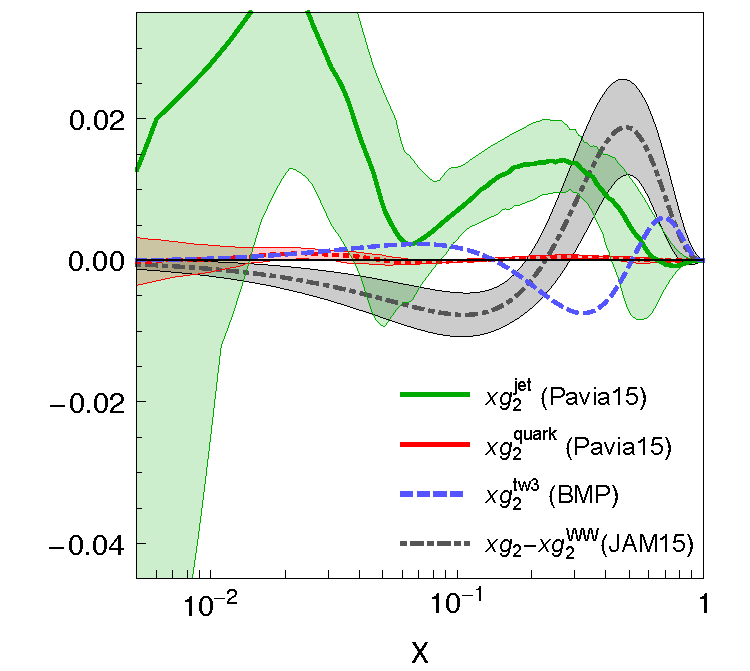
\includegraphics[width=8cm]{g2contrib}
\caption{\label{f:g2contrib} 
Different contributions to the $g_2$ structure function. 
}
\end{center}
\end{figure}

\begin{itemize}
\item large-$x$: bridges Braun's pure twist-3 theory and the data
\item samller-$x$: consttrains the small-$x$ behavior of transversity.
\end{itemize}



Another consequence of the new chiral odd term induced by the non-vanishing of
the chiral condensate on the non perturbative vacuum is that the
Burkardt-Cottingham sum rule is broken: 
\begin{align}
  \label{eq:BC}
  \int dx\, g_2(x) = \frac{\mj-m_q}{\Lambda} \int dx\, h_1(x) \ ,
\end{align}
where the integral over $h_1$ is related to target's tensor charge.
Consequences:
\begin{itemize}
\item Inclusive DIS become sensitive to the tensor charge; furthermore, teh BC summ rule isolates the effects due to the chiral odd part of the jet correlator. 
\item Both the jet mass $\mj$ and the tensor charge can in principle be calculated on the lattice
\item Comparison to the Burkhardt-Cottingham sum rule can provide experimental verification of lattice calculation
\item in turn these can be used to determine the size of the $h_1$ term in $g_2-g_2^{WW}$ and allow an eperimental extraction of the pure twist-3 terms.
\end{itemize}

It is important to explore in which other process does $\mj$ contribute, as to provide an experimental check of the formalism:
\begin{itemize}
\item inclusive $\Lambda$ production in $e^+ + e^-$
\item same-side dihadrons in $e^+ + e^-$ 
\end{itemize}
\todo{It would be cool to find a process where the $\mj$ contribution is th eonly one (similar to the BC breaking) ...}   


\section{Conclusions}

\noindent
------------------------------------------------- \\
Edited down to here\\
--------------------------------------------------\\


%%%%%%%%%%%%%%%%%%%%%%%%%%%%%%%%%%%%%%%%%%%%%%%%%%%%%%%%%%%%%%%%%%%%%%%%%
\section{Conclusions}


%%%%%%%%%%%%%%%%%%%%%%%%%%%%%%%%%%%%%%%%
%%%%%%%%% ACKNOWLEDGMENTS %%%%%%%%%%%%%%
%%%%%%%%%%%%%%%%%%%%%%%%%%%%%%%%%%%%%%%%

\begin{acknowledgments}
This work was supported by DOE contract No. DE-AC05-06OR23177,
under which Jefferson Science Associates, LLC operates Jefferson Lab, by the DOE contract DE-SC008791 and 
by the Joint Research Activity ``Study of Strongly
Interacting Matter'' (acronym HadronPhysics3, Grant Agreement No. 283286) under
the 7th Framework Programme of the European Community.
\end{acknowledgments}


\bibliographystyle{myrevtex}
\bibliography{mybiblio}

\end{document}
